\chapter{Implementation and Results}
\label{ch:chapter_five}%
% The \label{...}% enables to remove the small indentation that is generated, always leave the % symbol.

The whole work has been done in Matlab and Simulink and the overall scheme is represented in Figure \ref{fig:SIMULINK complete Model}

\begin{figure}
    \centering
    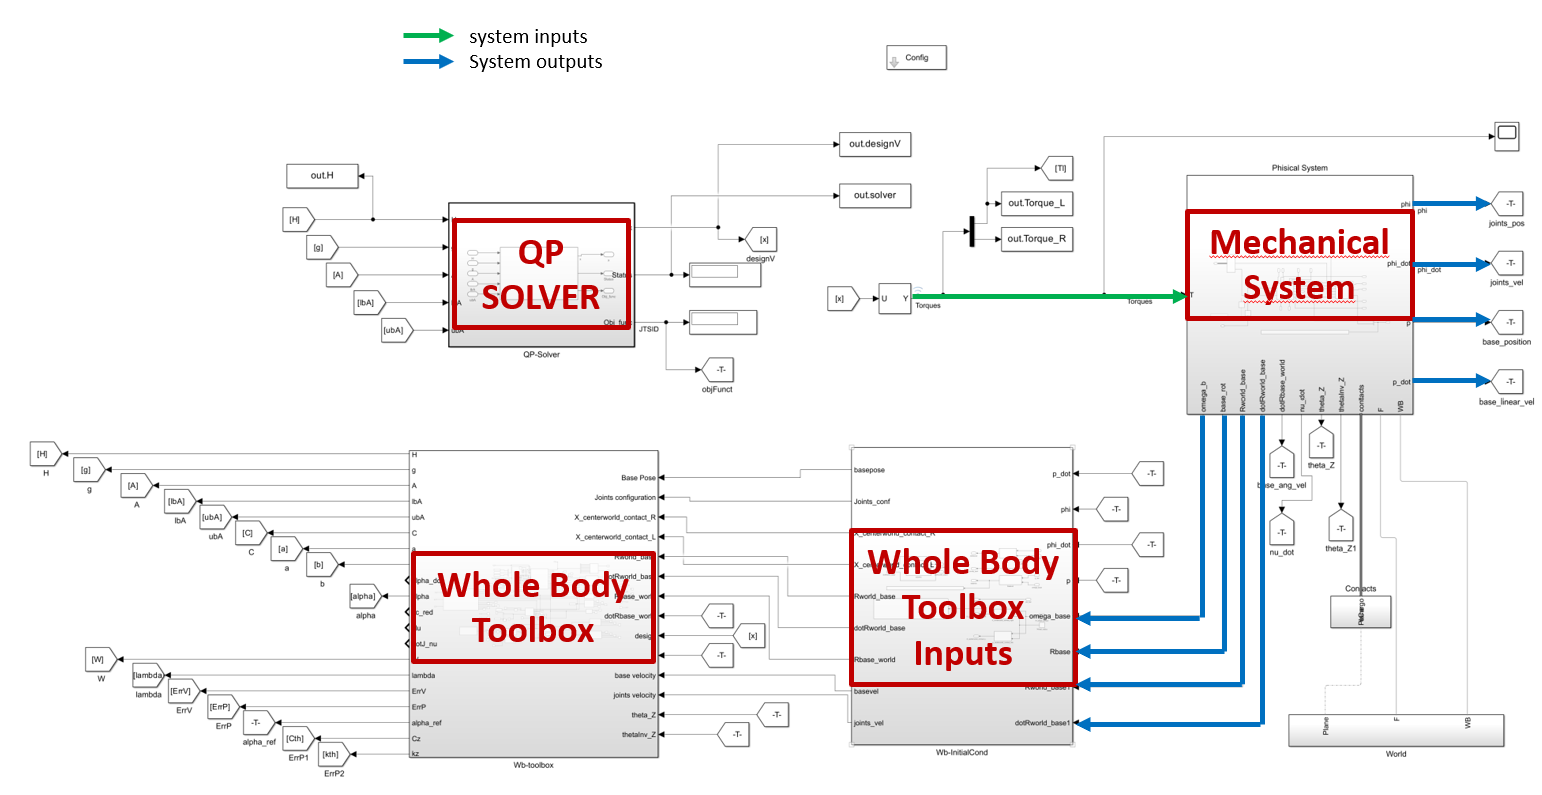
\includegraphics[width=1\linewidth]{Simulink overall model.png}
    \caption{Simulink complete Model.}
    \label{fig:SIMULINK complete Model}
\end{figure}

\section{Simulink modeling}
\label{sec:Simulink modeling}

Without going into the details of all the sub-systems involved, it can be useful to have a look to some specific blocks that have been used for modeling, sensing and control.
The simulation results reported in this chapter consider the E-Cargo loaded at its maximum capacity, with a total mass of 60 kg, and assuming a friction coefficient $\mu_c = 0.5$ between the wheels and the terrain.

\subsection{Robot URDF model}
\label{subsec:Robot URDF model}

\begin{figure}
  \centering
  \begin{minipage}{0.35\textwidth}
    \centering
    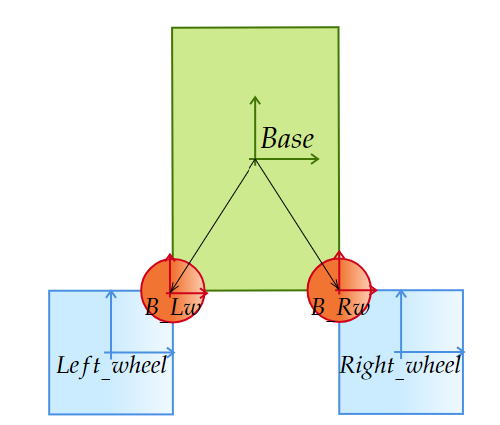
\includegraphics[width=1\linewidth]{Robot URDF model.png} % Adjust width as needed
  \end{minipage}%
  \begin{minipage}{0.55\textwidth}
    \small % Reduce font size for URDF code
    \begin{verbatim}
    <?xml version="1.0"?>
    <robot name="E-Cargo">
    
      <link name="base"> ... </link>
      <link name="left_wheel"> ... </link>
      <link name="right_wheel"> ... </link>
    
      <joint name="base_left" type="revolute"> ... </joint>
      <joint name="base_right" type="revolute"> ... </joint>
    
    </robot>
    \end{verbatim}
  \end{minipage}
  \caption{Robot URDF model.}
  \label{fig:Robot URDF model}
\end{figure}

The most important input of the simulation is the robot URDF file: an XML-based file format used to describe robots, humanoids in particular. It defines the structure, visual appearance, and physical properties of a robot's components such as links and joints with the assumption of rigid links and ideal joints already discussed in \cref{subsec: Links and Joints}.
Figure \ref{fig:Robot URDF model} provides a simplified sketch illustrating our URDF model, depicting a body with two wheels connected via two revolute joints. 
This input file is used both to create the robot block diagram in Simulink (as shown in Figure \ref{fig:Robot block diagram}), and to compute in real time all the matrices describing its dynamic through a Simulink toolbox named \textbf{Whole-Body Toolbox (Wb-Toolbox)}.

\begin{figure}
    \centering
    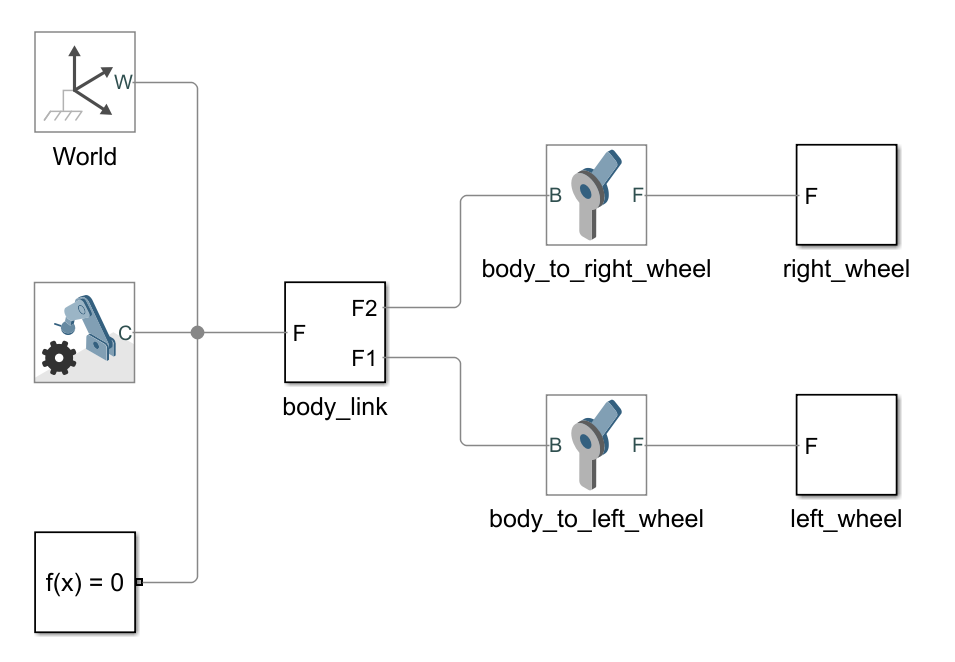
\includegraphics[width=0.5\linewidth]{Robot Block Diagram.png}
    \caption{Robot block diagram.}
    \label{fig:Robot block diagram}
\end{figure}

\subsection{Simulink blocks overview}
\label{subsec:Simulink blocks overview}

Once the robot has been created in the simulation environment, its contacts with the external world have been defined through the Simscape block \textit{Spatial Contact Force} (Figure \ref{fig:Spatial Contact Force block}).

\begin{figure}
    \centering
    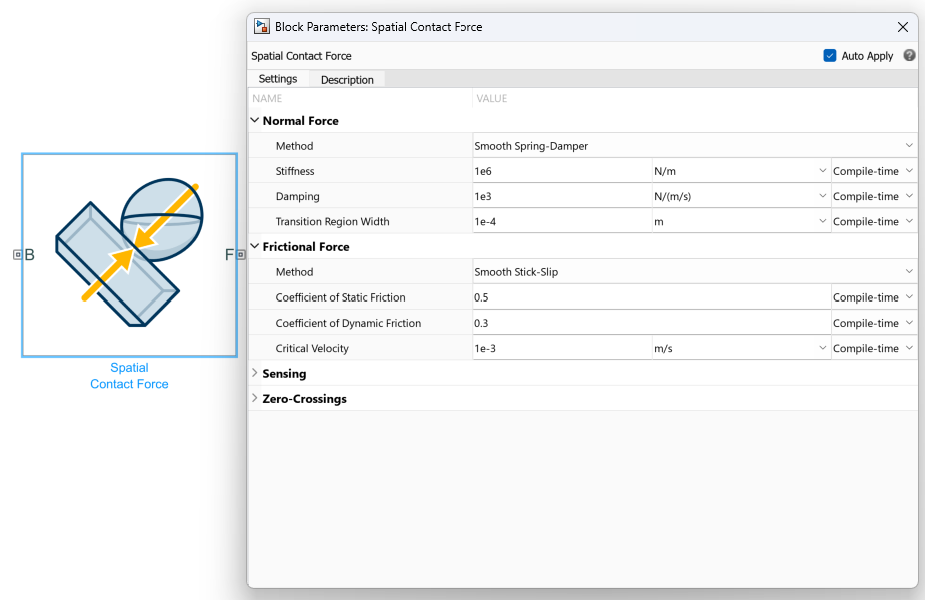
\includegraphics[width=0.7\linewidth]{Spatial Contact Force.png}
    \caption{Spatial Contact Force block.}
    \label{fig:Spatial Contact Force block}
\end{figure}

This block model the contact as rigids (spring-damper) coherently with our model assumption; in our simulation we assume just static friction between the wheels and the terrain for this moment, and the friction coefficient used as input for this block, is the same used for the friction cone constraint. 

The sensing of the all the needed reasonable feedbacks have been made through the block \textit{Transform Sensor}, (Figure \ref{fig:Transform Sensor Block}) which allows us to compute important time-dependent transformations between two frames named \textit{base} and \textit{follower}, and to project them in a third user-specified frame.
This last feature is very useful to change the representation switching from \textit{left trivialized}, \textit{right trivialized} and \textit{mixed}.

\begin{figure}
    \centering
    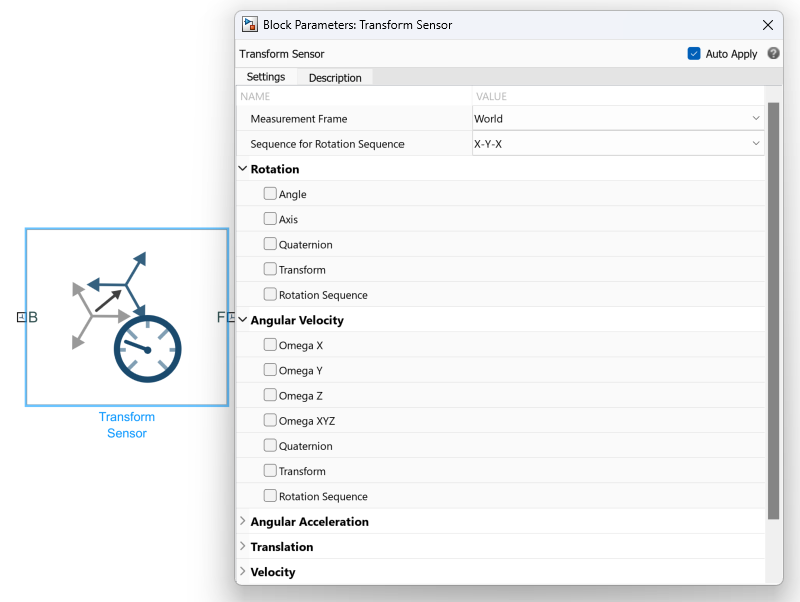
\includegraphics[width=0.7\linewidth]{Transform Sensor Block.png}
    \caption{Transform Sensor Block.}
    \label{fig:Transform Sensor Block}
\end{figure}

The last remark regards the block \textit{OSQP}: it uses the OSQP libraries to solve the optimization-based control problem given the inputs defined in \cref{sec:Converting Least-Squares to Quadratic Programming} and a maximum number of possible iterations.

\begin{figure}
    \centering
    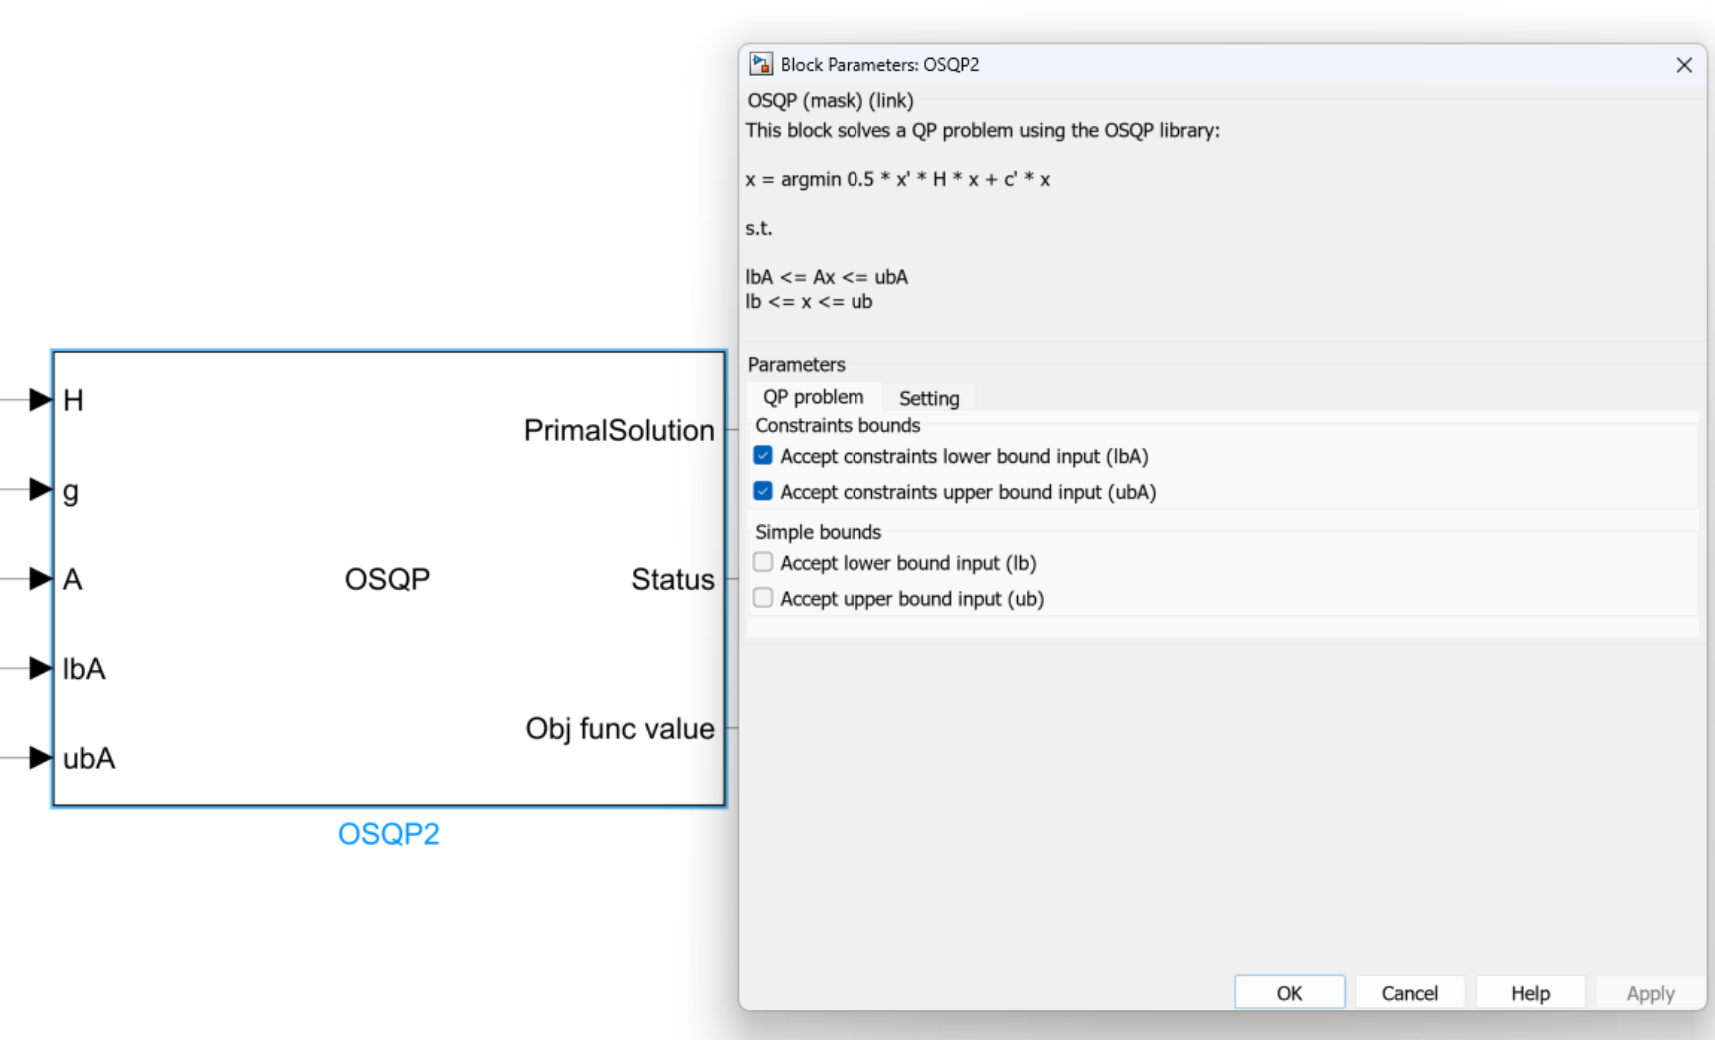
\includegraphics[width=0.8\linewidth]{OSQP.png}
    \caption{OSQP solver block.}
    \label{fig:OSQP solver block}
\end{figure}


\section{Simulation results}
\label{sec:Simulation results}

To validate our mathematical derivation of the controller we conducted some simulations involving different features that we want our E-Cargo to posses.
Simulating a real scenario, we found a set of parameters that, given the system model, does not change with respect to the different nominal trajectories and different requirements.

\subsection{Gain tuning}
\label{subsec:Gain tuning}

This type of controller requires proper tuning of certain user-defined parameters. In our case, we did not adopt a specific criterion for this; instead, we used a trial-and-error approach to find the best compromise between the initial swing-up performance of the E-Cargo and effective trajectory tracking.

\begin{table}[h!]
\centering
\setlength{\tabcolsep}{30pt} % Adjust the value to increase the distance
\large
\begin{tabular}{>{\bfseries}l l}
\textbf{Parameter} & \textbf{Value} \\
\hline
\multicolumn{2}{l}{\textit{TSID Controller Parameters}} \\
\hline
$K_{P\alpha_x}$ & 80 \\
$K_{P\alpha_x}$ & 80 \\
$K_{P\theta}$ & 100 \\
$K_{D\alpha_x}$ & 113.14 \\
$K_{D\alpha_x}$ & 113.14 \\
$K_{D\theta}$ & 70.7 \\
\hline
\multicolumn{2}{l}{\textit{QP Weights}} \\
\hline
$w_{\alpha_x}$ & 100 \\
$w_{\alpha_y}$ & 100 \\
$w_{\tau}$ & 1 \\
$w_{\xi}$ & 1 \\
$w_{\delta}$ & 1 \\
$\lambda$ & $1^{-3}$ \\
\hline
\multicolumn{2}{l}{\textit{PI Trajectory Planner}} \\
\hline
$K_{Pp}$ & 0.5 \\
$K_{Ip}$ & 0.1 \\
\end{tabular}
\caption{Set of Gains and Weights.}
\label{tab:Set of Gains and Weights}
\end{table}

\newpage
Given the set of parameters in Table \ref{tab:Set of Gains and Weights}, three different cases have been simulated:

\begin{enumerate}
    \item initial swing-up starting from $\theta = 25^{\circ}$

    With the same nominal trajectories in the $x$ direction, (Figure \ref{fig:Nominal trajectories x-direction}) two different nominal trajectories in the $y$ direction:
    \item nominal $y$ trajectory $=0$
    \item nominal $y$ trajectory $= A \sin{t}$
\end{enumerate}

\begin{figure}
    \centering
    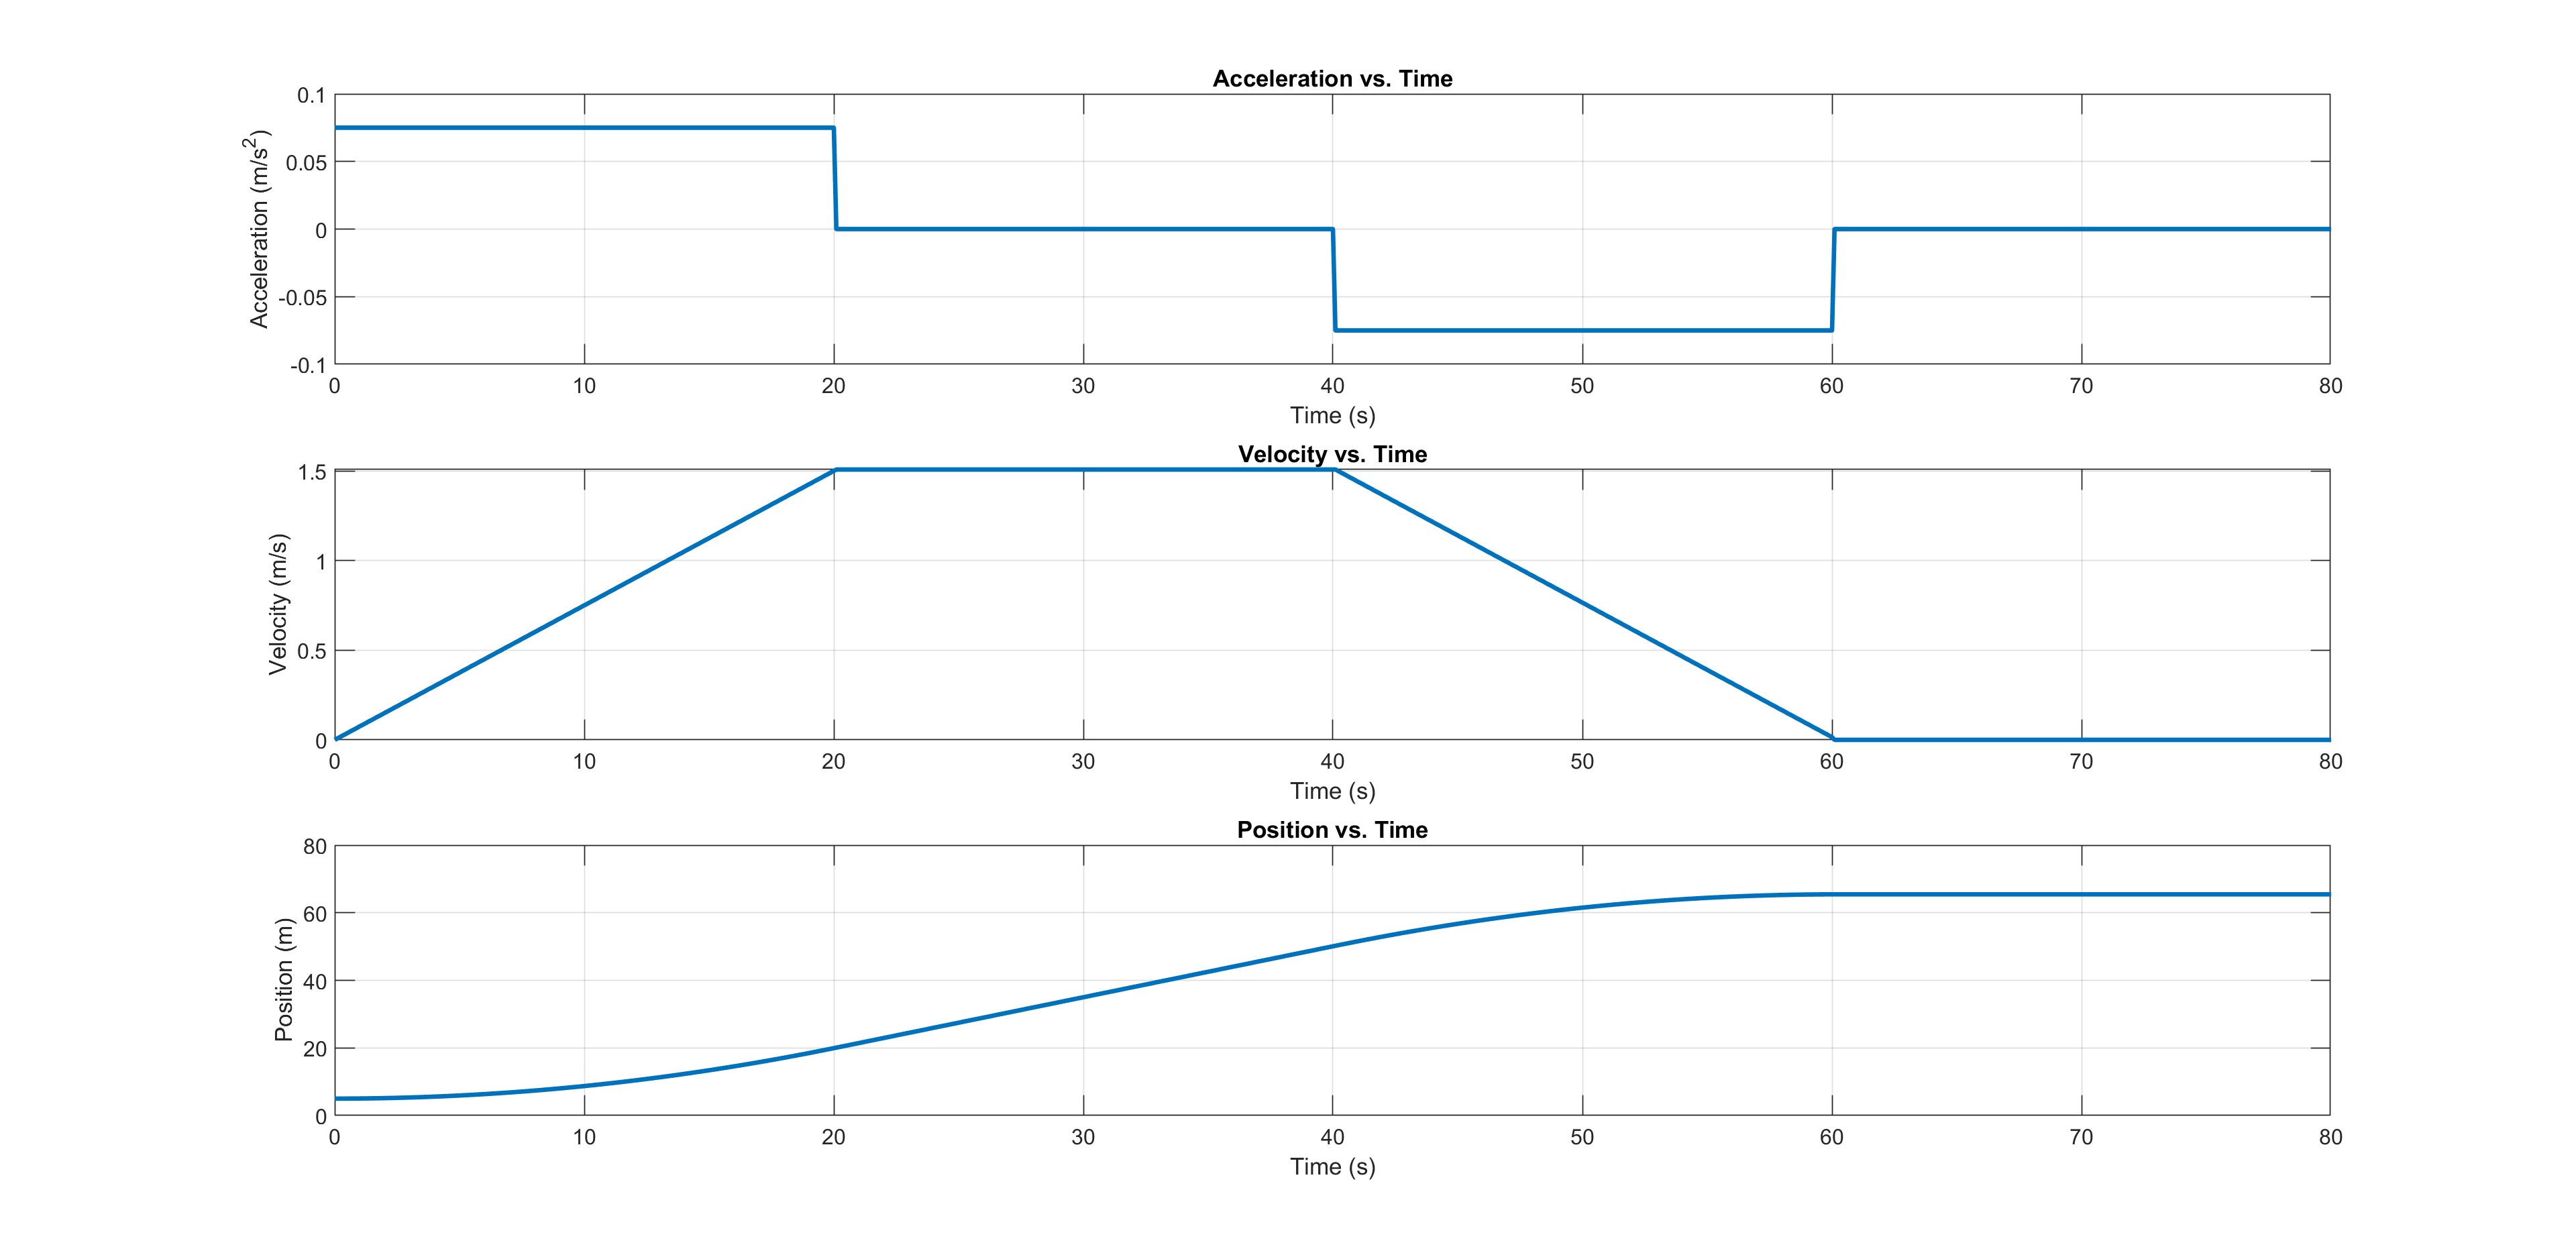
\includegraphics[width=1\linewidth]{Images/x-trajectory/Reference_trajectories.jpg}
    \caption{Nominal trajectories x-direction.}
    \label{fig:Nominal trajectories x-direction}
\end{figure}

The trajectory shown in Figure \ref{fig:Nominal trajectories x-direction} has been used to evaluate the controller's performance in the key phases: start, acceleration, deceleration, and stop; considering a cruise velocity of 1.5 $m/s$ which is close to the maximum allowed one.

\subsection{Swing-up}
\label{subsec:Swing-up}

The swing-up has been tested using nominal trajectories where the initial position of the control point is set with zero velocity and acceleration. Additionally, the nominal pitch angle velocity and acceleration are also set to zero.

In Figure \ref{fig:Swing-Up Position error} are shown in red the actual trajectories in position, while in blue are shown the nominal ones:
After a transient of $\approx$ 4 sec, the red curves follow the blue ones.

Figure \ref{fig:Swing-Up Velocity error} shows the velocity trajectories, using the same color criteria. It can be observed how the error between the actual and nominal velocities regulates the nominal pitch angle trajectory shown in Figure \ref{fig:Swing-Up Position error}.

\begin{figure}
    \centering
    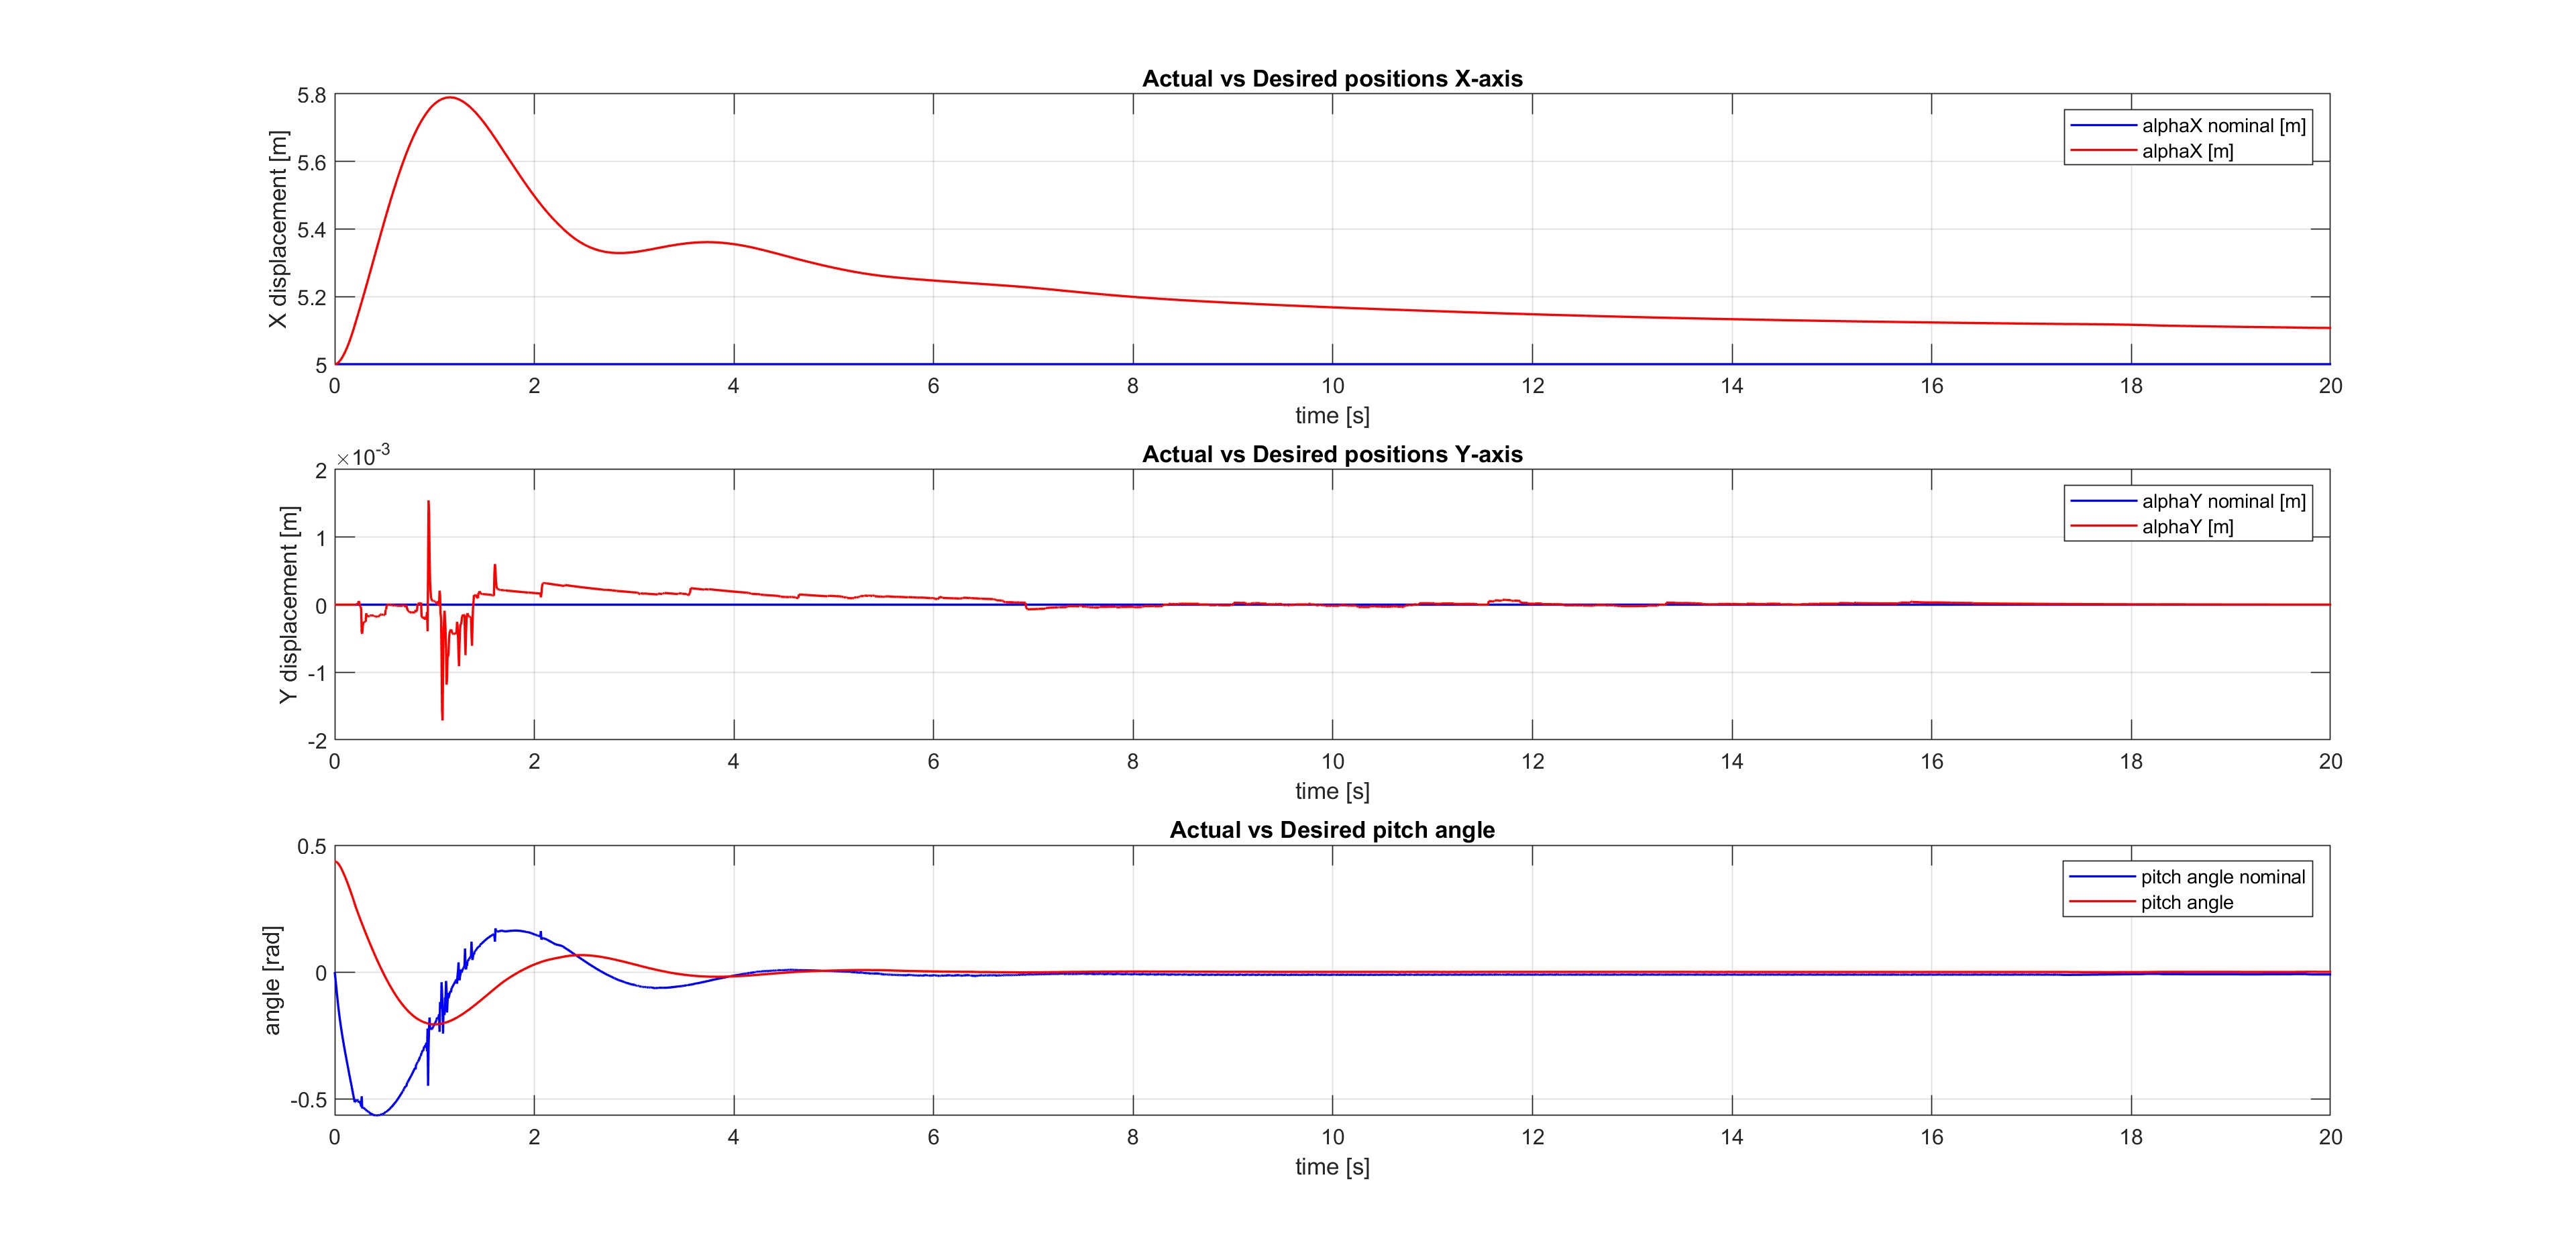
\includegraphics[width=1\linewidth]{Images/Swing-Up/Position_error.jpg}
    \caption{Swing-Up Position error.}
    \label{fig:Swing-Up Position error}
\end{figure}

\begin{figure}
    \centering
    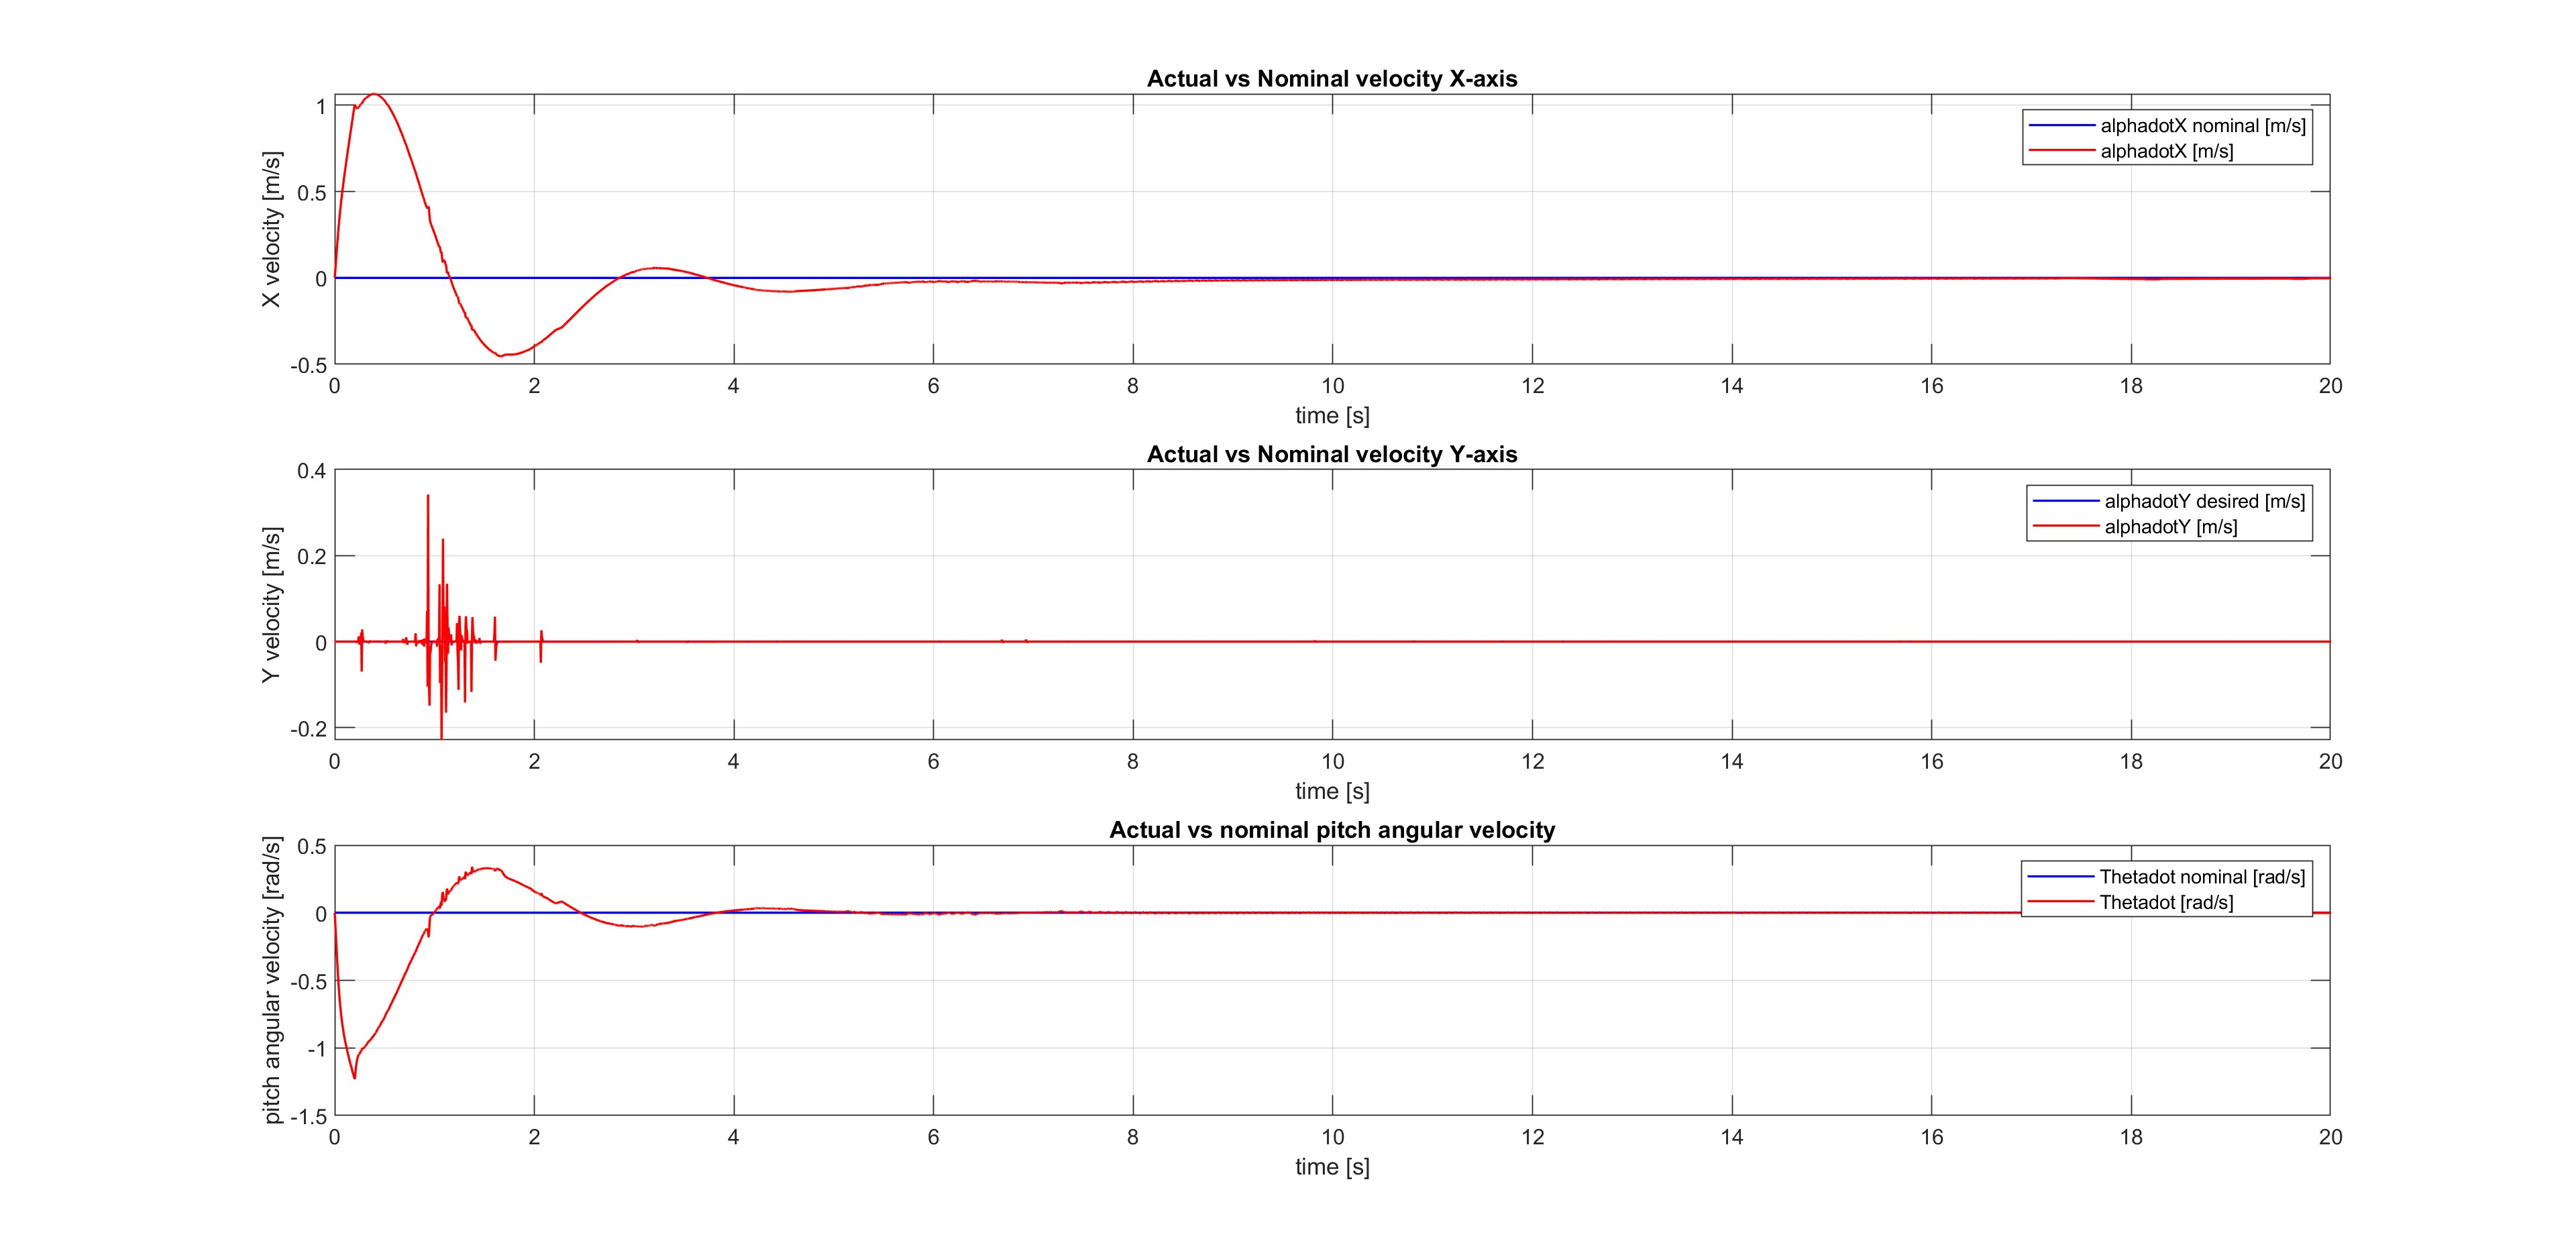
\includegraphics[width=1\linewidth]{Images/Swing-Up/Velocity_error.jpg}
    \caption{Swing-Up Velocity error.}
    \label{fig:Swing-Up Velocity error}
\end{figure}

\subsection{Straight Trajectory}
\label{subsec:Straight Trajectory}

The tracking has been tested by starting with the base in its upright position $\theta^{n} = 0$, considering that this is more difficult with respect to start with a pitch angle >0.

Apart for some mismatches corresponding to the points in which the acceleration profile is discontinuous, the red actual trajectories follows the nominal blue ones both in position (Figure\ref{fig:Straight trajectory Position error}) and in velocity (Figure\ref{fig:Straight trajectory Velocity error}).

\begin{figure}
    \centering
    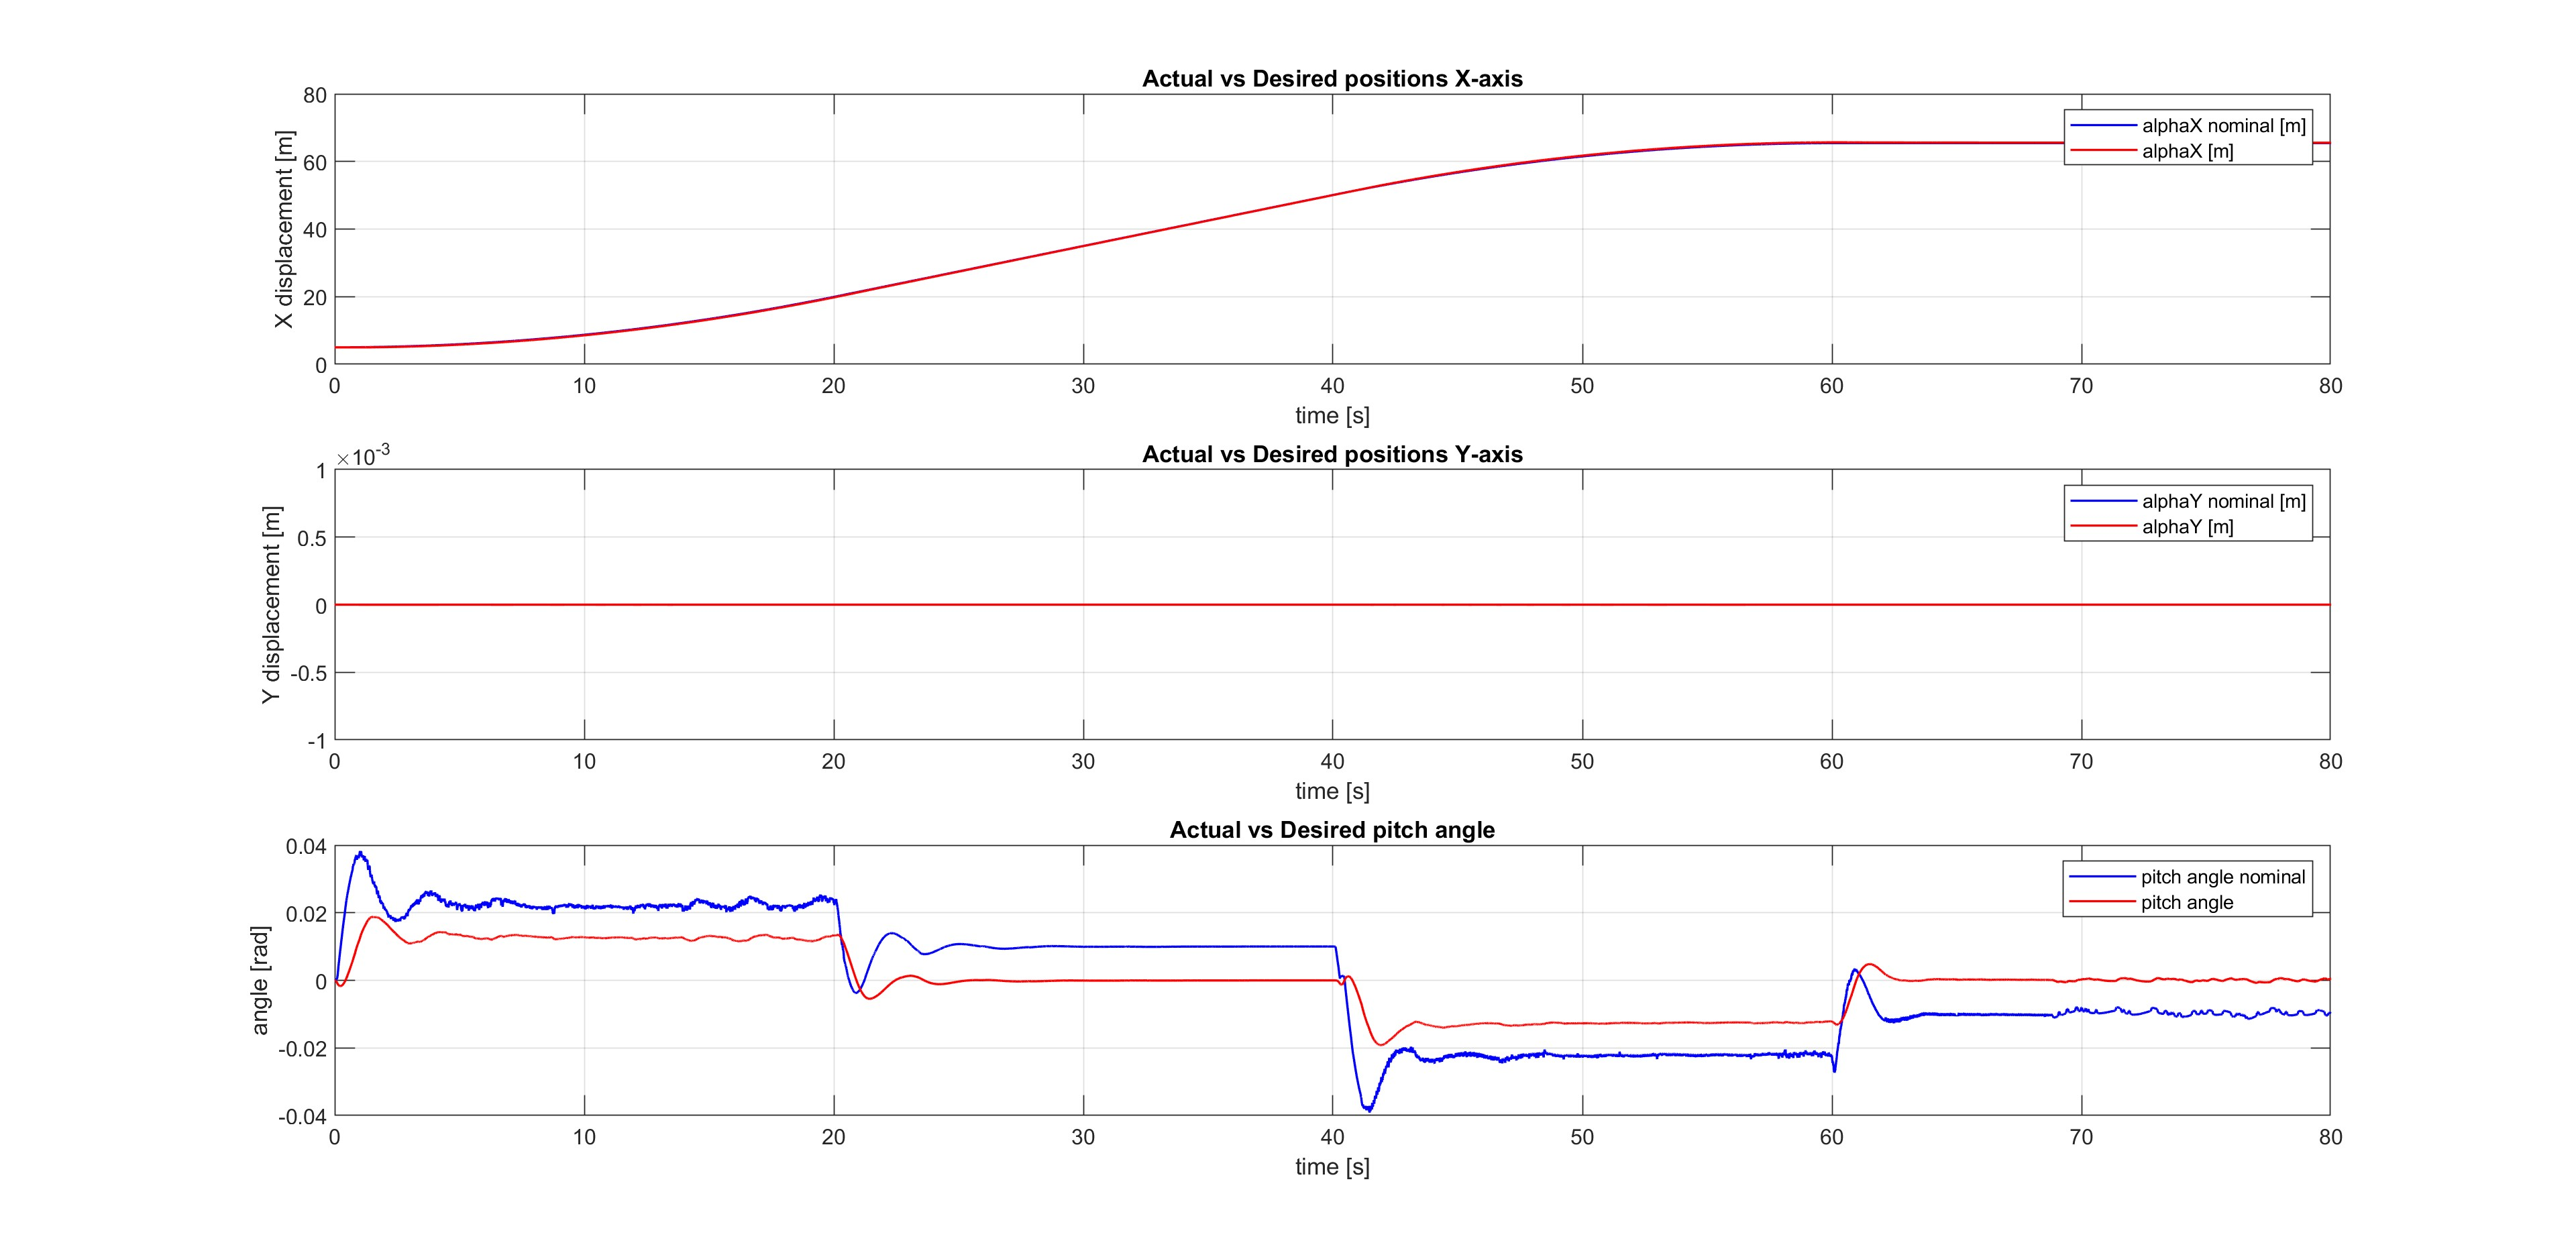
\includegraphics[width=1\linewidth]{Images/x-trajectory/Position_error.jpg}
    \caption{Straight trajectory Position error.}
    \label{fig:Straight trajectory Position error}
\end{figure}

\begin{figure}
    \centering
    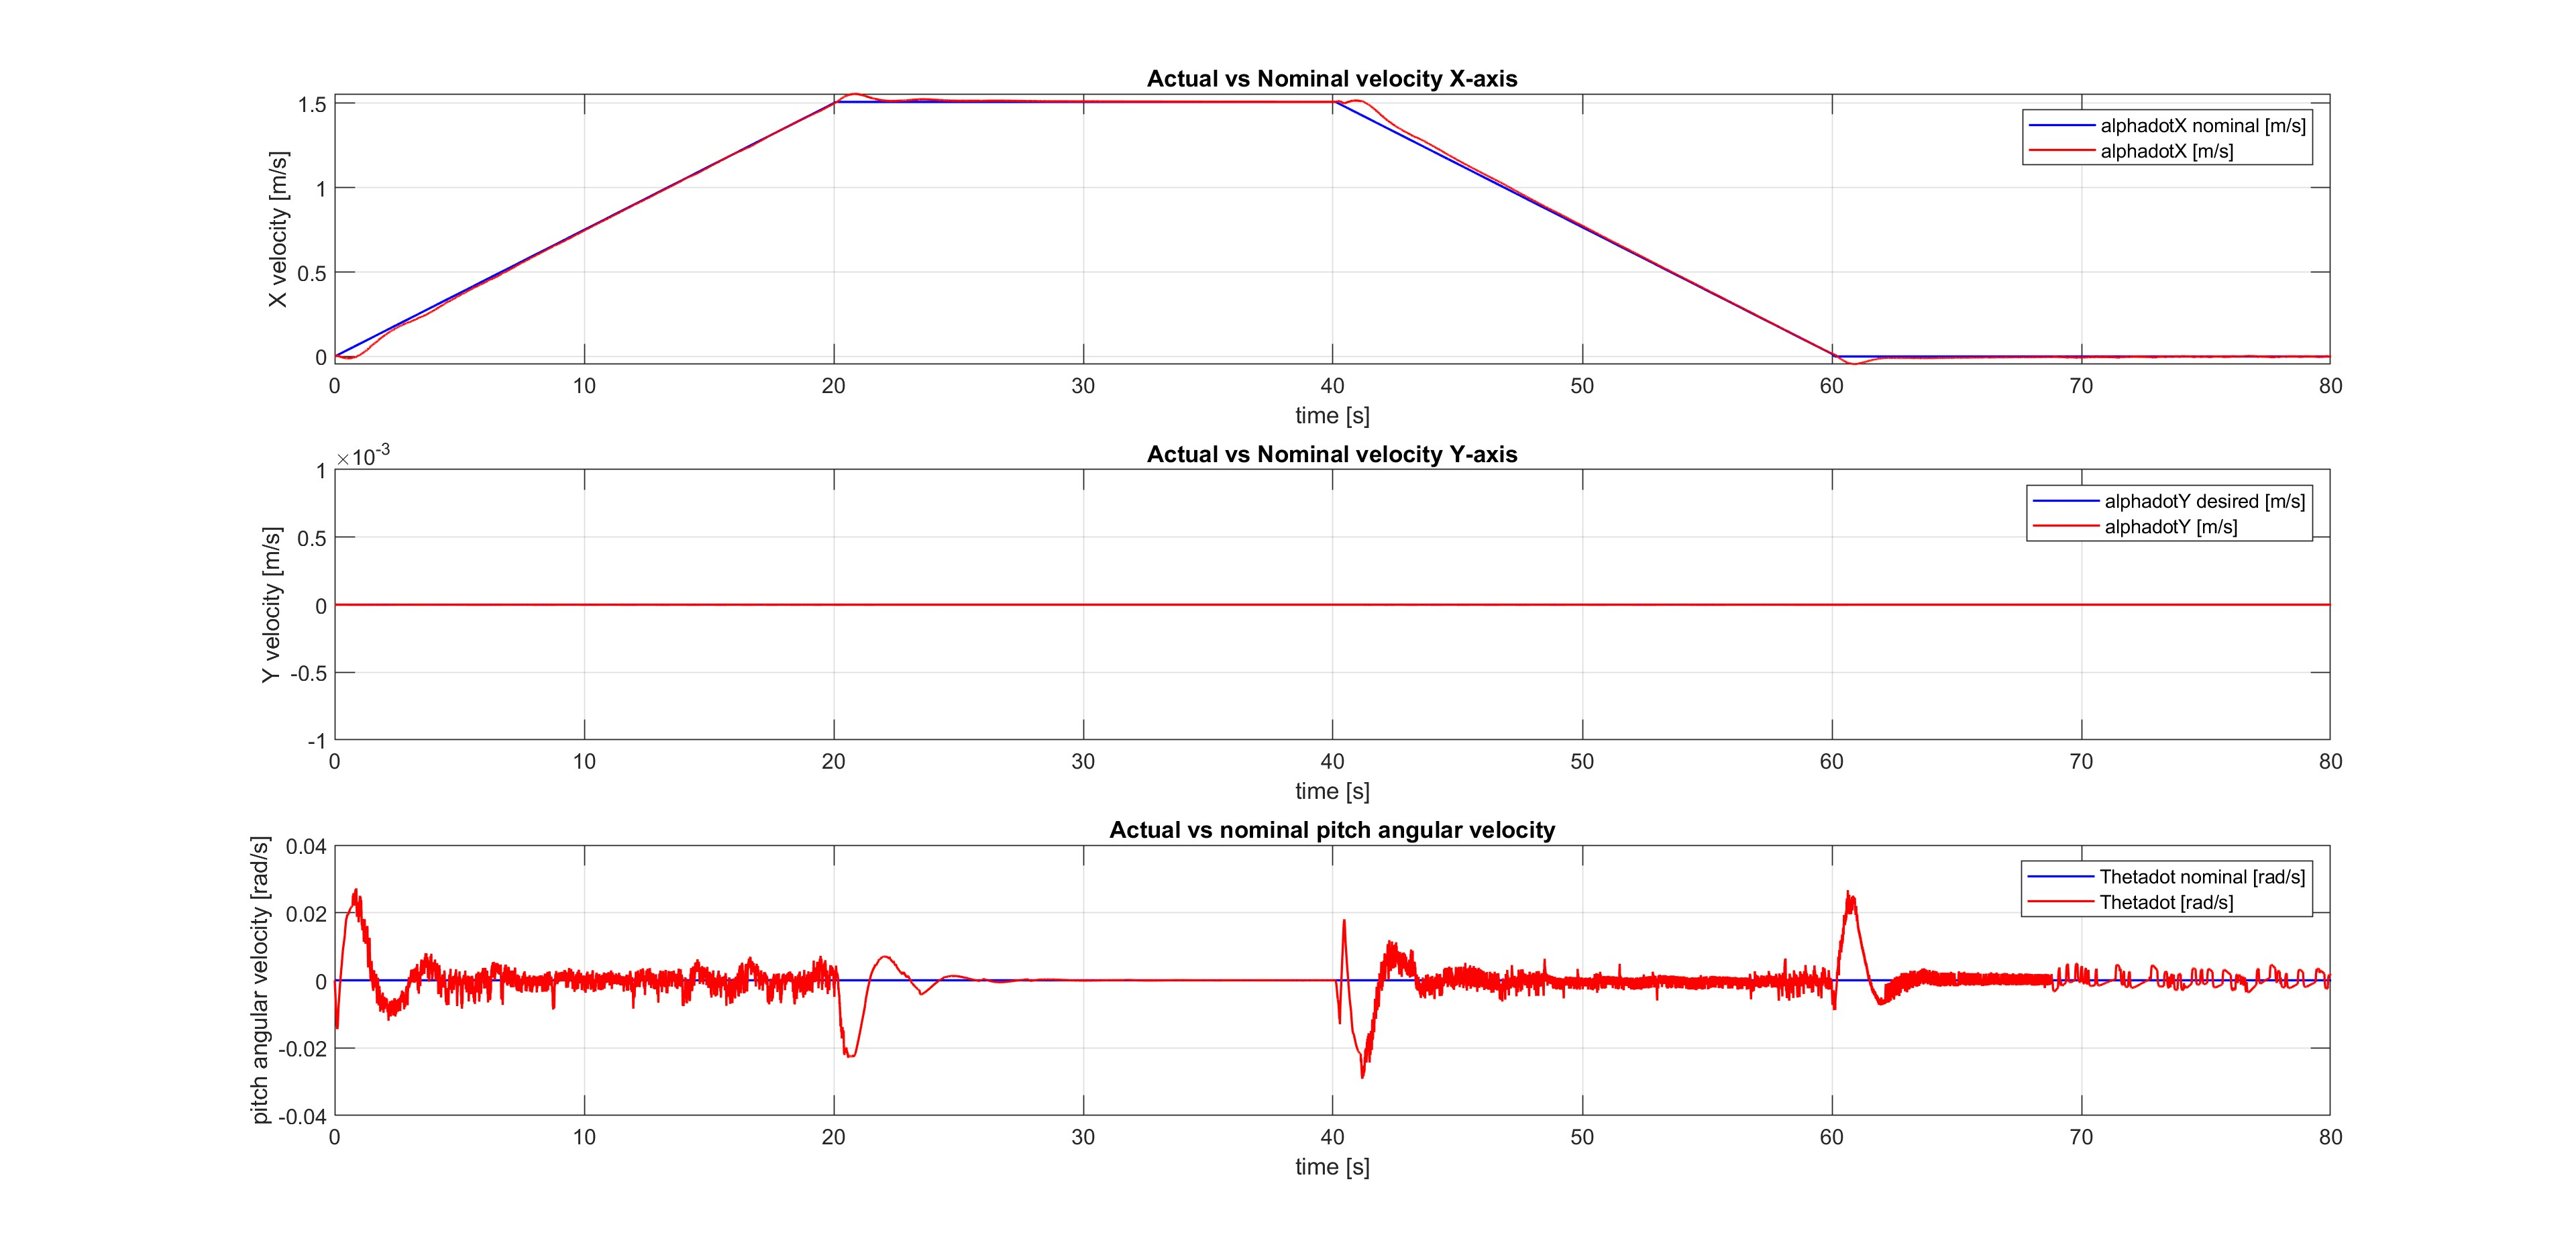
\includegraphics[width=1\linewidth]{Images/x-trajectory/Velocity_error.jpg}
    \caption{Straight trajectory Velocity error.}
    \label{fig:Straight trajectory Velocity error}
\end{figure}

\subsection{Sinusoidal Trajectory}
\label{subsec:Sinusoidal Trajectory}

To validate the decision regarding the choice of controlling a point different from the base, allowing for instantaneous velocity components along the y-axis, we tested a final trajectory involving a general sinusoidal nominal trajectory in the y direction.

\begin{figure}
    \centering
    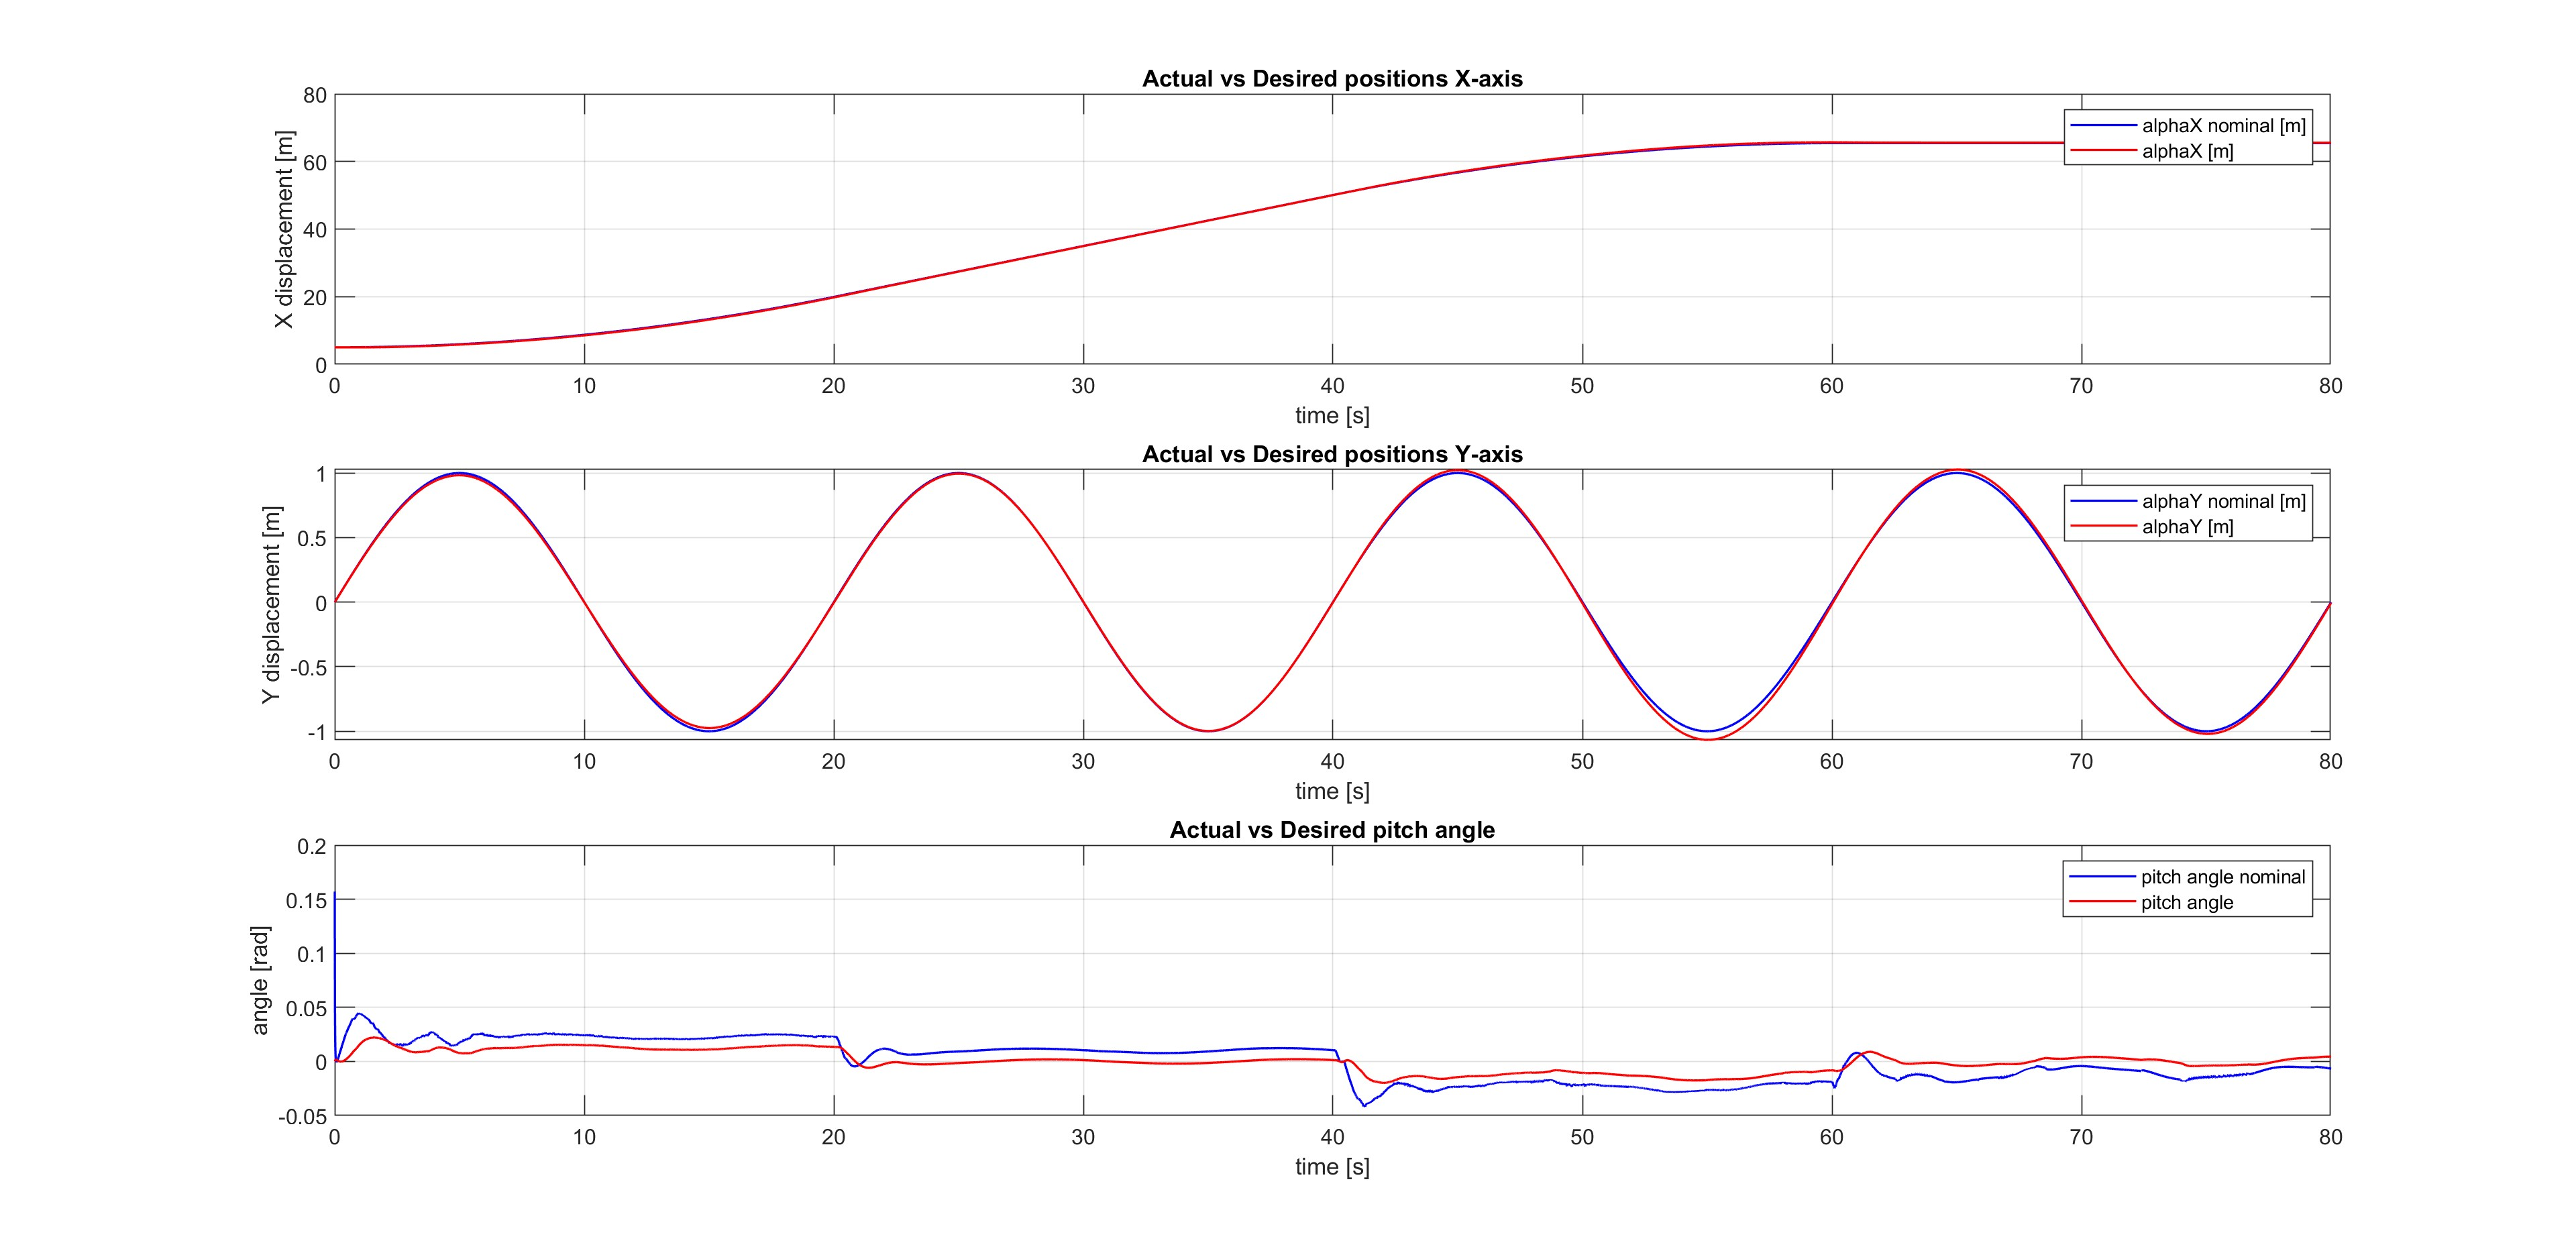
\includegraphics[width=1\linewidth]{Images/sine trajectory/Position_error.jpg}
    \caption{Sinusoidal trajectory Position error.}
    \label{fig:Sinusoidal trajectory Position error}
\end{figure}

\begin{figure}
    \centering
    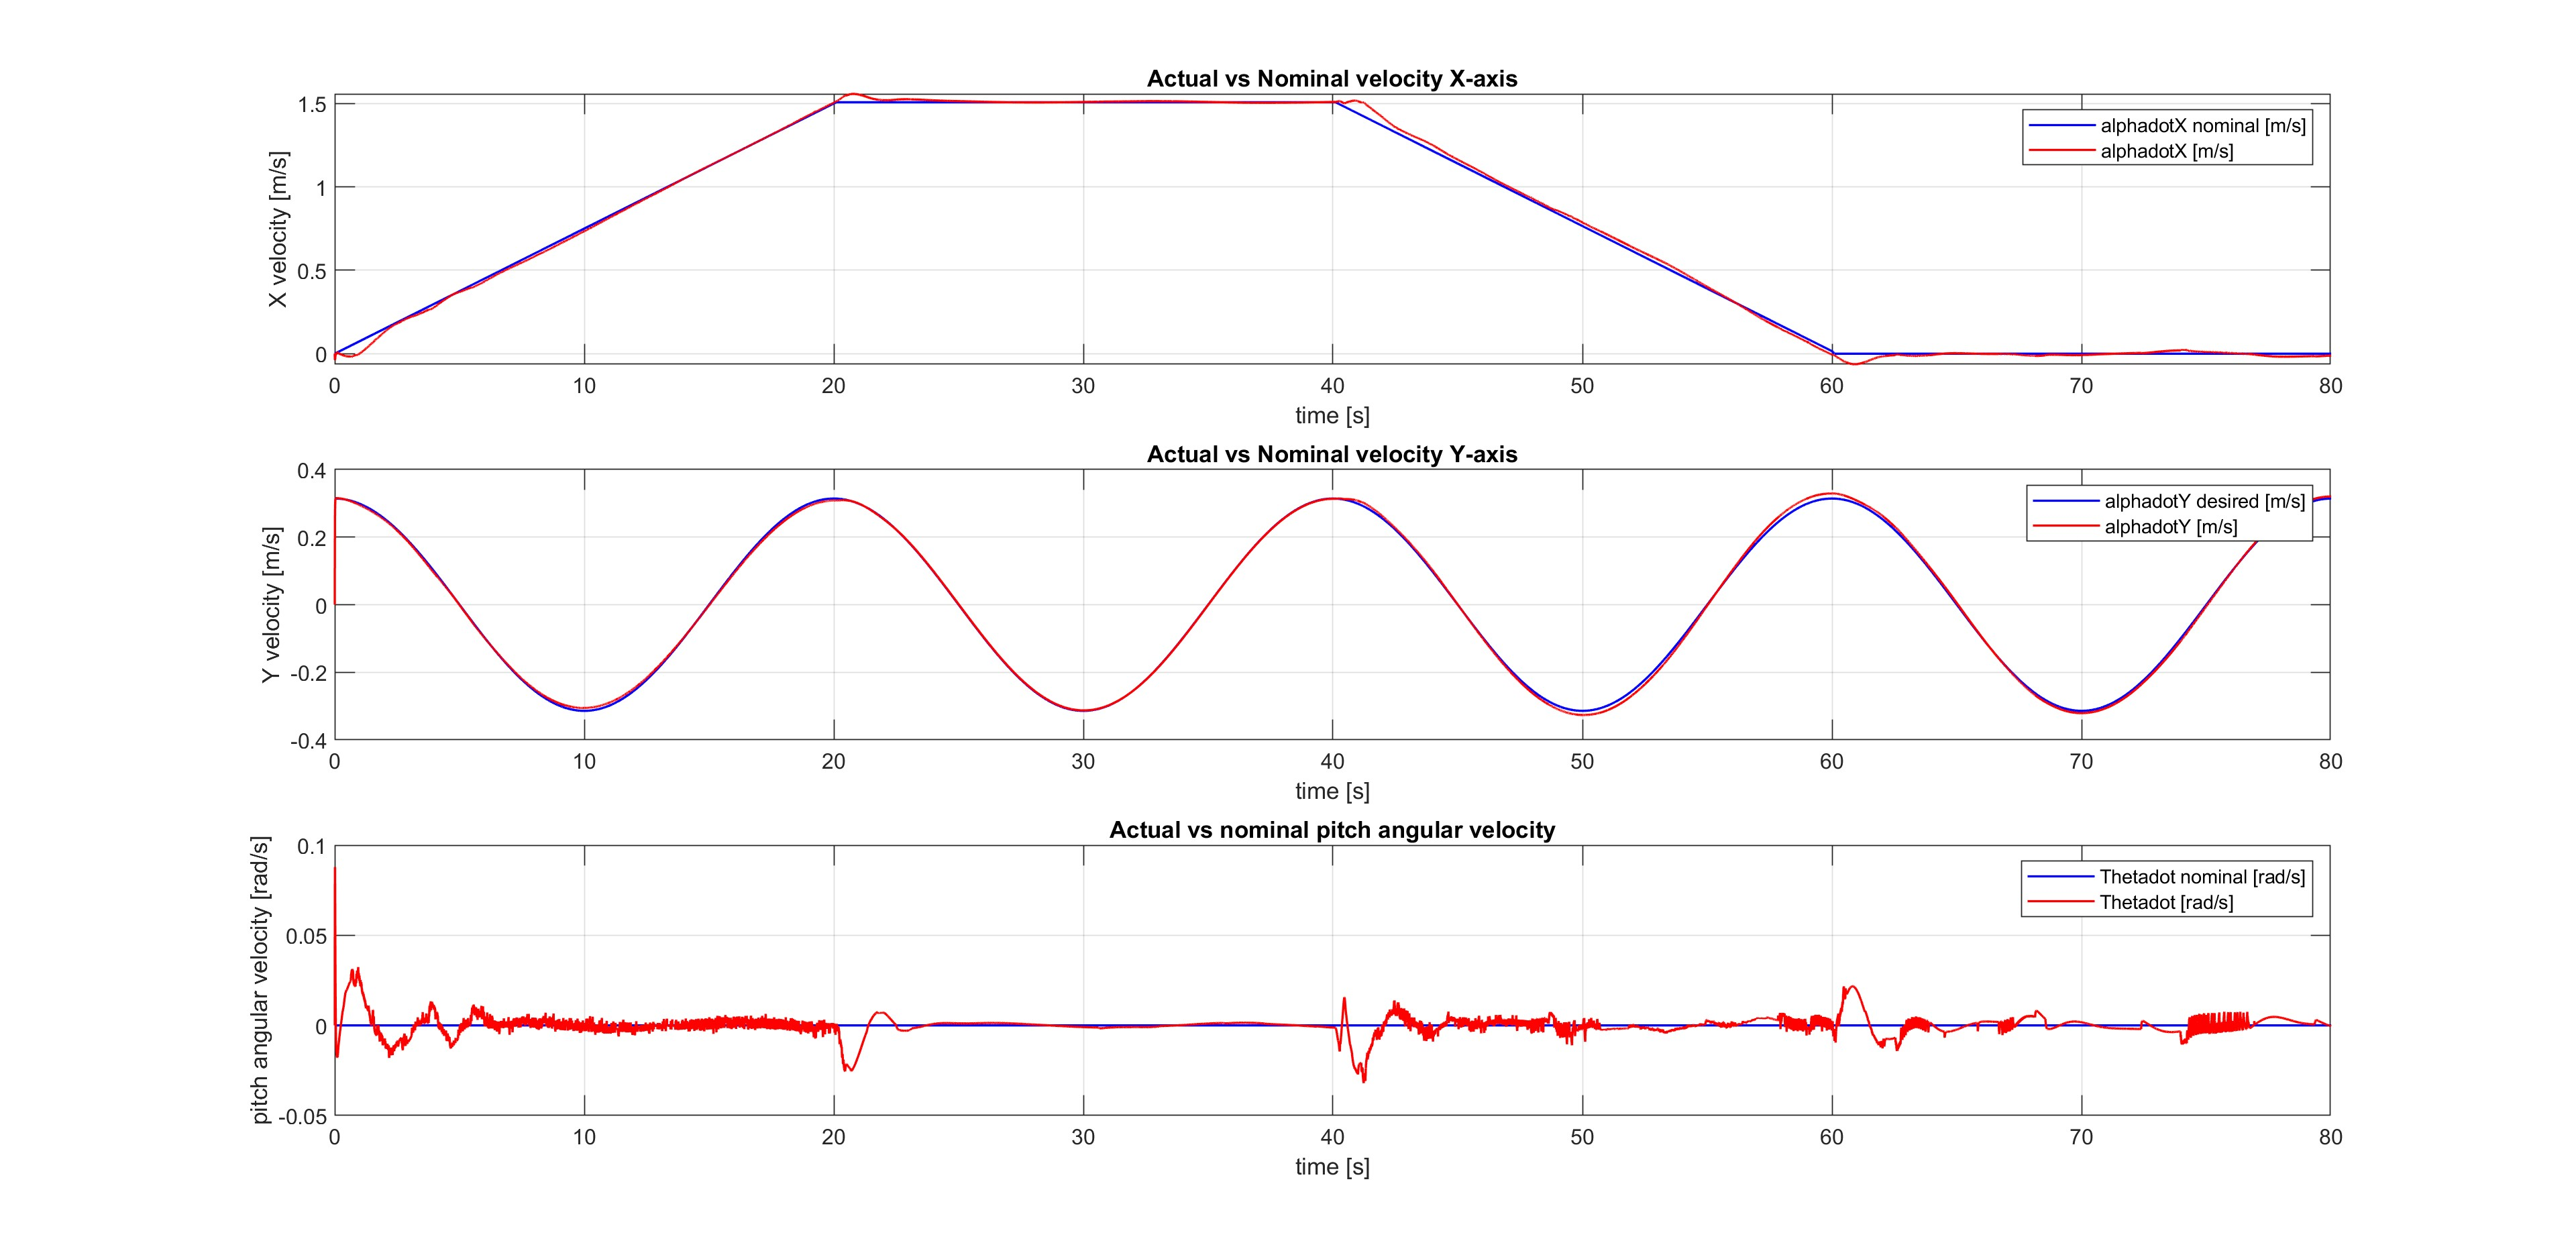
\includegraphics[width=1\linewidth]{Images/sine trajectory/Velocity_error.jpg}
    \caption{Sinusoidal trajectory Velocity error.}
    \label{fig:Sinusoidal trajectory Velocity error}
\end{figure}

Also in this last case the actual red curves follow the nominal blue ones both in position (Figure\ref{fig:Sinusoidal trajectory Position error}) and in velocity (Figure\ref{fig:Sinusoidal trajectory Velocity error}). 



